\documentclass[xcolor=dvipsnames, aspectratio = 169]{beamer}
\usepackage[english]{babel} %% english
\usepackage[utf8]{inputenc}
\usepackage[T1]{fontenc}
\usepackage{include/chariteBeamer}
\usepackage{hyperref}
\author[E. Sprünken]{Erin Sprünken}
\institute[]{
Institut für Biometrie und Klinische Epidemiologie\\[1Ex] 
Charité - Universitätsmedizin Berlin, Berlin\\[1Ex]
erin-dirk.spruenken@charite.de} 
\titlegraphic{\pgfuseimage{frontUnilogo}}

\tikzset{>=latex}
%\usepackage{amsmath}
%\usetikzlibrary{shadows}
\usepackage[edges]{forest}
\usetikzlibrary{positioning}
\usepackage{biostat}
\setbeamertemplate{caption}[numbered]
\let\qed\relax
\forestset{declare toks={elo}{}}
%% ================================================================== %% 

\author[L. Mödl, M. Becher, E. Sprünken]{Lukas Mödl, Matthias Becher, Erin Sprünken} 
\title{R-Kurs: Tag 1} 
\date[]{\today}

%% ================================================================== %% 
\setbeamercolor*{mycol}{bg=chariteGray, fg=chariteBlue}

\hyphenation{Sam-ples}
\begin{document}

%% ================================================================== %%
%% ================================================================== %%
\setbeamertemplate{footline}{\begin{tikzpicture}
    \node [inner sep=0pt, anchor=east] (0,0) {
      
\includegraphics[width=\paperwidth,height=0.7cm]{include/charite_footer}};
    \node [inner sep=0pt, anchor=east] at (-0.5ex,-0ex){};
\end{tikzpicture}}

\setbeamertemplate{headline}{
%\leavevmode
\hspace{-0.49em}\hbox{
	\begin{beamercolorbox}[wd=1.02\paperwidth,ht=2.25ex,dp=1ex,left]{mycol}%
    \usebeamerfont{section in head/foot}
  \end{beamercolorbox}%
}}
{
  \usebackgroundtemplate{ \hspace{-0.5em}\begin{tikzpicture}
  \node[opacity=0.7, anchor=south] (0,0) {
\includegraphics[height=\paperheight, width=1.04\paperwidth]{include/frontmatter.pdf}};
  \end{tikzpicture}
} 
%\frame{\titlepage}
\begin{frame}
\centering
	\vspace{4em}
	{\Large \textcolor{chariteBlue}{\inserttitle}}\\
	 \vspace{1em}
	{\Large \textcolor{black}{\insertauthor \\}} 
	\vspace{2em}
	{\footnotesize \textcolor{black}{\insertinstitute \\\vspace{1em} \insertdate}} 
	\vspace{0em}
	\begin{figure}[h!]
		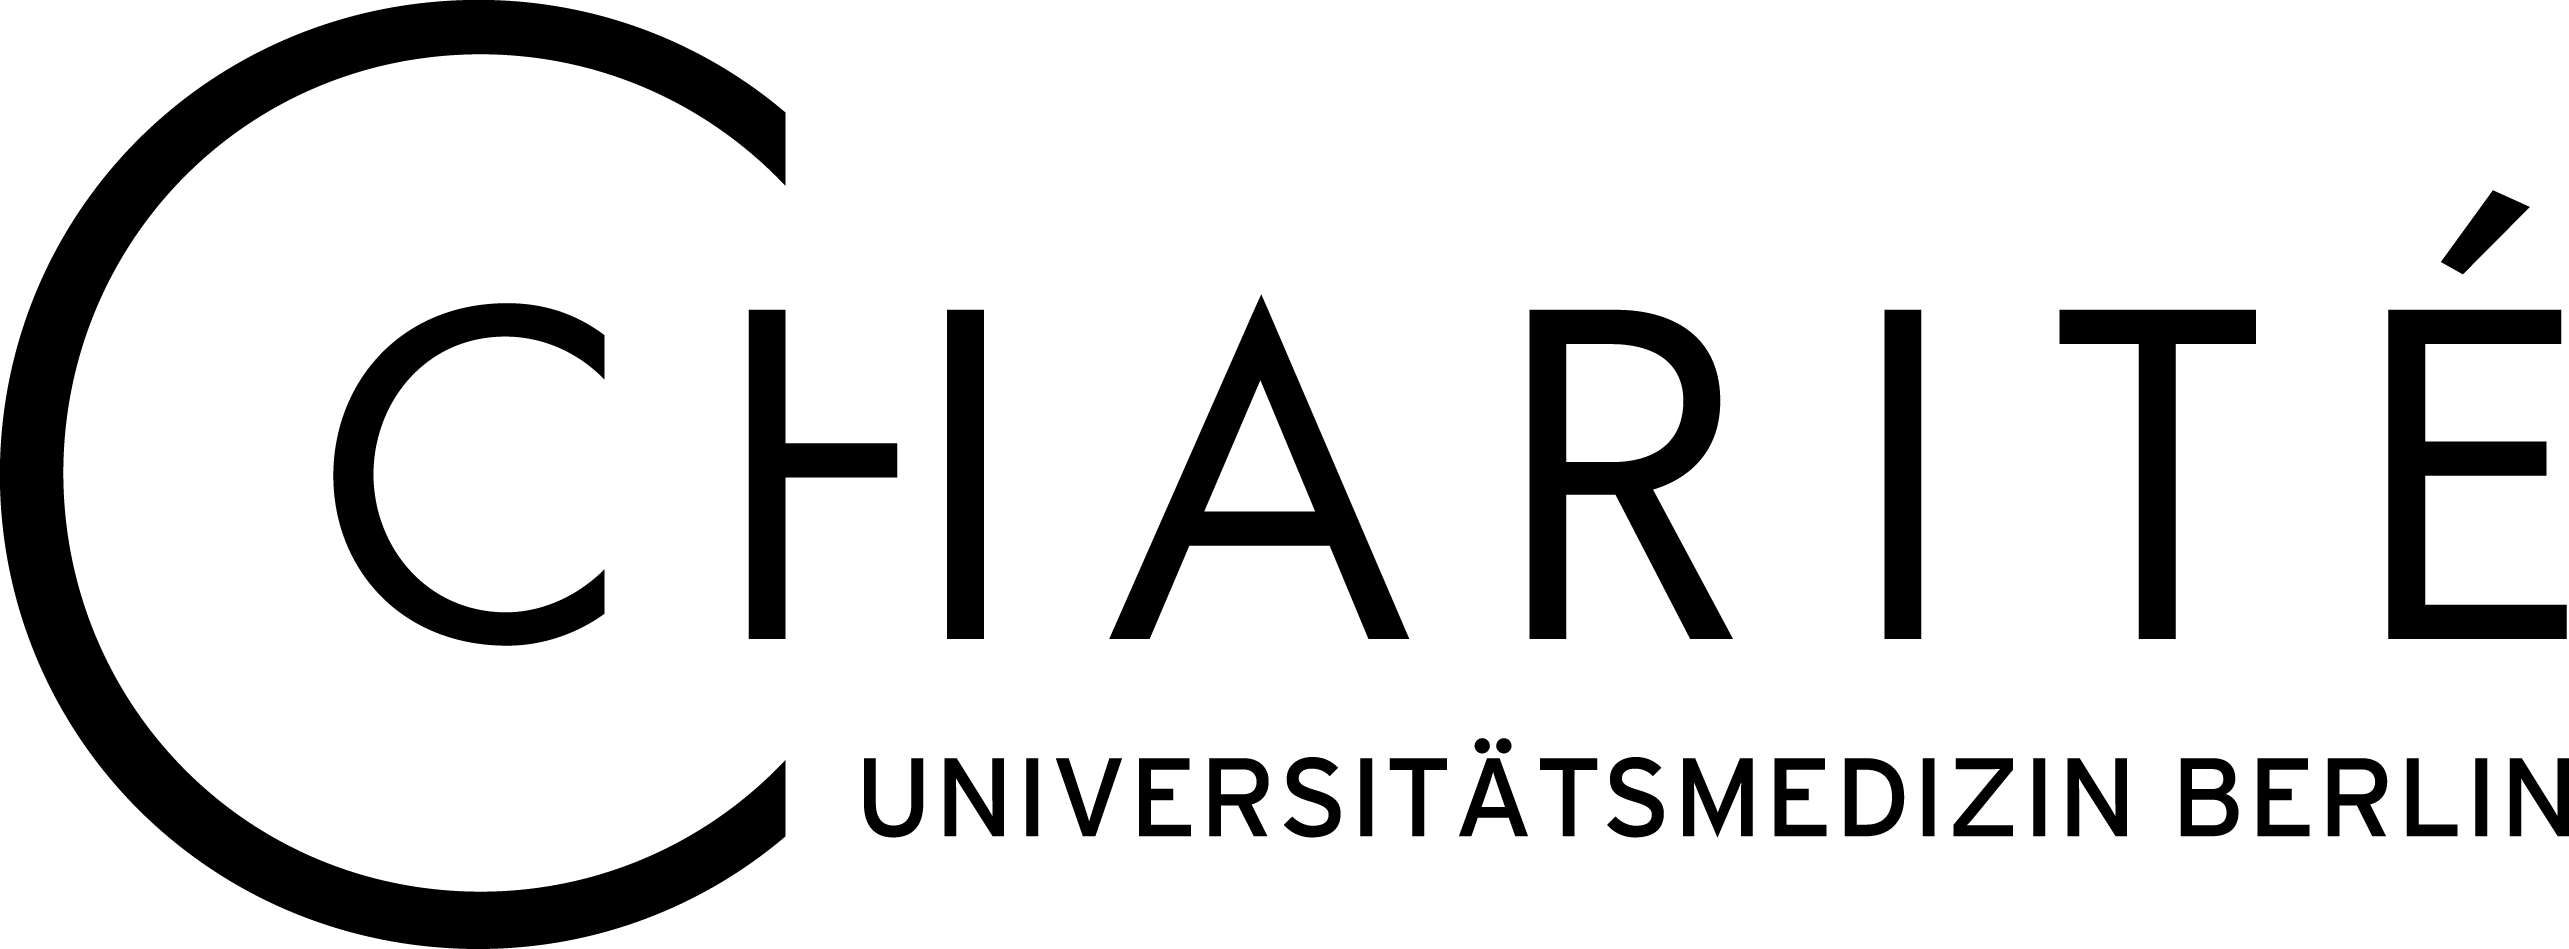
\includegraphics[width=5cm]{include/Charite_Logo.png}
	\end{figure}
%	\pgfuseimage{frontUnilogo}
\end{frame}
}
%% ================================================================== %%

\setbeamertemplate{footline}{\begin{tikzpicture}
    \node [inner sep=0pt, anchor=east] (0,0) {
      
\includegraphics[width=\paperwidth,height=0.7cm]{include/charite_footer}};
    \node [inner sep=0pt, anchor=east] at (-0.5ex,-0ex) {\tiny \insertframenumber{}$\,$|$\,$\inserttotalframenumber};
\end{tikzpicture}}

\setbeamertemplate{headline}{%
%\leavevmode%
\hspace{-0.49em}\hbox{
	\begin{beamercolorbox}[wd=.68\paperwidth,ht=2.25ex,dp=1ex,left]{mycol}%
    \usebeamerfont{section in head/foot}\hspace*{1em}
  \end{beamercolorbox}%
  \begin{beamercolorbox}[wd=.20\paperwidth,ht=2.25ex,dp=1ex,right]{mycol}%
    \usebeamerfont{author in head/foot}\insertshortauthor
  \end{beamercolorbox}%
  \begin{beamercolorbox}[wd=.14\paperwidth,ht=2.25ex,dp=1ex,center]{mycol}%
    \usebeamerfont{date in head/foot}\insertdate
  \end{beamercolorbox}%
  }
}


\frame{\tableofcontents}

\setbeamertemplate{headline}{%
%\leavevmode%
\hspace{-0.49em}\hbox{
	\begin{beamercolorbox}[wd=.68\paperwidth,ht=2.25ex,dp=1ex,left]{mycol}%
    \usebeamerfont{section in head/foot}\hspace*{1em}\thesection. \  \insertsectionhead
  \end{beamercolorbox}%
  \begin{beamercolorbox}[wd=.20\paperwidth,ht=2.25ex,dp=1ex,right]{mycol}%
    \usebeamerfont{author in head/foot}\insertshortauthor
  \end{beamercolorbox}%
  \begin{beamercolorbox}[wd=.14\paperwidth,ht=2.25ex,dp=1ex,center]{mycol}%
    \usebeamerfont{date in head/foot}\insertdate
  \end{beamercolorbox}%
  }
}

\section{Einführung}
\begin{frame}[fragile]{Motivation}
  \begin{itemize}
  \item Statistische Analysen
  \item Handlungsspielraum verglichen mit SPSS, SAS, Stata
  \item Open Source
  \end{itemize}
%  \begin{tikzpicture}
%  [[level distance=11mm,
%  every node/.style = {shape=rectangle, rounded corners,
%    draw, align=center,
%    top color=white, bottom color=blue!20}]]
%  \node {Sample}
%		child { node {Group 1} }
%		child { node {Group i}
%			child { node {Observation 1 (Cluster 1)} }
%			child { node {Observation j (Cluster j)} }
%			child { node {Observation $n_i$ (Cluster $n_i$)} }
%		 }
%		child { node {Group n} };
%\end{tikzpicture}
\end{frame}
%\begin{frame}[fragile]{Data Structure}
%%\begin{forest}
%%for tree={s sep+=3.9em,circle,draw,inner sep=1pt,
%%    where n children=0{fill=white}{fill=black},
%%    decision edge label/.style n args=3{
%%    edge label/.expanded={node[midway,auto=#1,anchor=#2,\forestoption{elo}]{\strut$#3$}}
%%  },
%%  decision/.style={if n=1
%%    {decision edge label={left}{east}{#1}}
%%    {decision edge label={right}{west}{#1}}
%%  },
%%    }
%% [,label=above:{Samples}
%%  [,label=above:{Group $1$}
%%   %[,label=above:{Cluster $[1,n_1]$}
%%    %[,label=below:{Obs $1$}]
%%    %[,label=below:{Obs $k$}]
%%    %[,label=below:{Obs $n_{11m}$}]
%%   %]
%%  ]
%%  [,label=above:{Group $i$}
%%	[,label=above:{Cluster $1$}
%%    	[,label=below:{Obs $1$}]
%%    	[,label=below:{Obs $k$}]
%%    	[,label=below:{ Obs $m_{i1}$ }]
%%    ]
%%   	[,label=above:{Cluster $j$}
%%    	[name=X,label=below:{Obs $1$}] % \tikz{\node[] (unsichtbarenode1) {};}
%%    	[name=Y,label=below:{Obs $k$}] % \tikz{\node[] (unsichtbarenode2) {};}
%%    	[,label=below:{Obs $m_{ij}$}]
%%    	
%%    ]
%%   	[,label=above:{Cluster $n_i$}
%%    	[,label=below:{Obs $1$}]
%%    	[,label=below:{Obs $k$}]
%%   		[,label=below:{Obs $m_{in_i}$}]
%%    ]
%%  ]
%%  [,label=above:{Group $d$}
%%   %[,label=above:{Cluster $[1,n_n]$}
%%    %[,label=below:{Obs $1$}]
%%    %[,label=below:{Obs $k$}]
%%    %[,label=below:{Obs $n_{11m}$}]
%%   %]
%%  ]
%% ]
%% %\draw (Y.south) -- (X.south);
%%\end{forest}
%\begin{center}
%\begin{tikzpicture}[align=center, parent anchor=south,child anchor=north,grow=south, level 1/.style={sibling distance=9em, level distance = 4em},
%level 2/.style={sibling distance=6em}, 
%level 3/.style={sibling distance=4em}, level distance = 5em]
%%\tikzset{every node/.style={ball color=orange,circle,text=white}}
%\tikzset{every node/.style={rectangle, draw=black, rounded corners=0.5em, inner sep=2pt, minimum size = 3em, text width=3em, font=\scriptsize},
%level 4/.style={rectangle, draw=none, level distance=3.3em, text=red}}
%\tikzset{edge from parent/.style={draw,solid,thick,black}}
%\node {Sample}
%	child {node (v1){Group 1} edge from parent[child anchor=north east]}
%	child {node[draw=none] (v1left){\Large $\cdots$} edge from parent[draw=none]}
%	child {node (v2){Group i}
%		child {node (v11){Cluster 1}
%			child {node (v111){Obs 1}}
%			child {node (v112){Obs k}}
%			child {node (v113){Obs $m_{i1}$}}
%		}
%		child {node[draw=none] (v11left){\Large $\cdots$} edge from parent[draw=none]}
%		child {node (v12){Cluster j}
%			child {node (v121){Obs 1}}
%			child {node (v122){Obs k}
%				child {node[draw=none] (v1221){$\rho$} edge from parent[draw=none]}			
%			}
%			child {node (v123){Obs $m_{ij}$}}
%		}
%		child {node[draw=none] (v11right){\Large $\cdots$} edge from parent[draw=none]}
%		child {node (v13){Cluster $n_i$}
%			child {node (v131){Obs 1}}
%			child {node (v132){Obs k}}
%			child {node (v133){Obs $m_{in_i}$}}
%		}
%	}
%	child {node[draw=none] (v1rightt){\Large $\cdots$} edge from parent[draw=none]}
%	child {node (v3){Group d} edge from parent[child anchor=north west]}
%;
%\path[draw=red,dotted, thick] (v121.south)  edge[bend right](v122.south);
%\path[draw=red,dotted, thick] (v122.south) edge[bend right](v123.south);
%\path[draw=red,dotted, thick] (v121.south) edge[bend right](v123.south);
%%\path[draw=black, dotted,very thick] (v1.east) edge (v2.west);
%%\path[draw=black, dotted,very thick] (v2.east) edge (v3.west);
%%\draw
%
%\end{tikzpicture}
%\end{center}
%\end{frame}


\begin{frame}{Installation}
	\begin{itemize}
		\item \href{https://www.r-project.org/}{R (Software)  
\includegraphics[scale=0.01]{include/r-logo}}
		\item \href{https://www.rstudio.com/}{RStudio (GUI = Graphical User Interface = Arbeitsumgebung)  
\includegraphics[scale=0.04]{include/rstudio-logo}}
		\item Alternativ (aber von uns nicht empfohlen): xcode, Visual Studio, Texteditor
	\end{itemize}
	
\end{frame}

%% ================================================================== %%
\section{Wie spreche ich mit R?}

\begin{frame}{Oberfläche von RStudio}
\begin{columns}[T]
	\begin{column}{0.6\textwidth}
	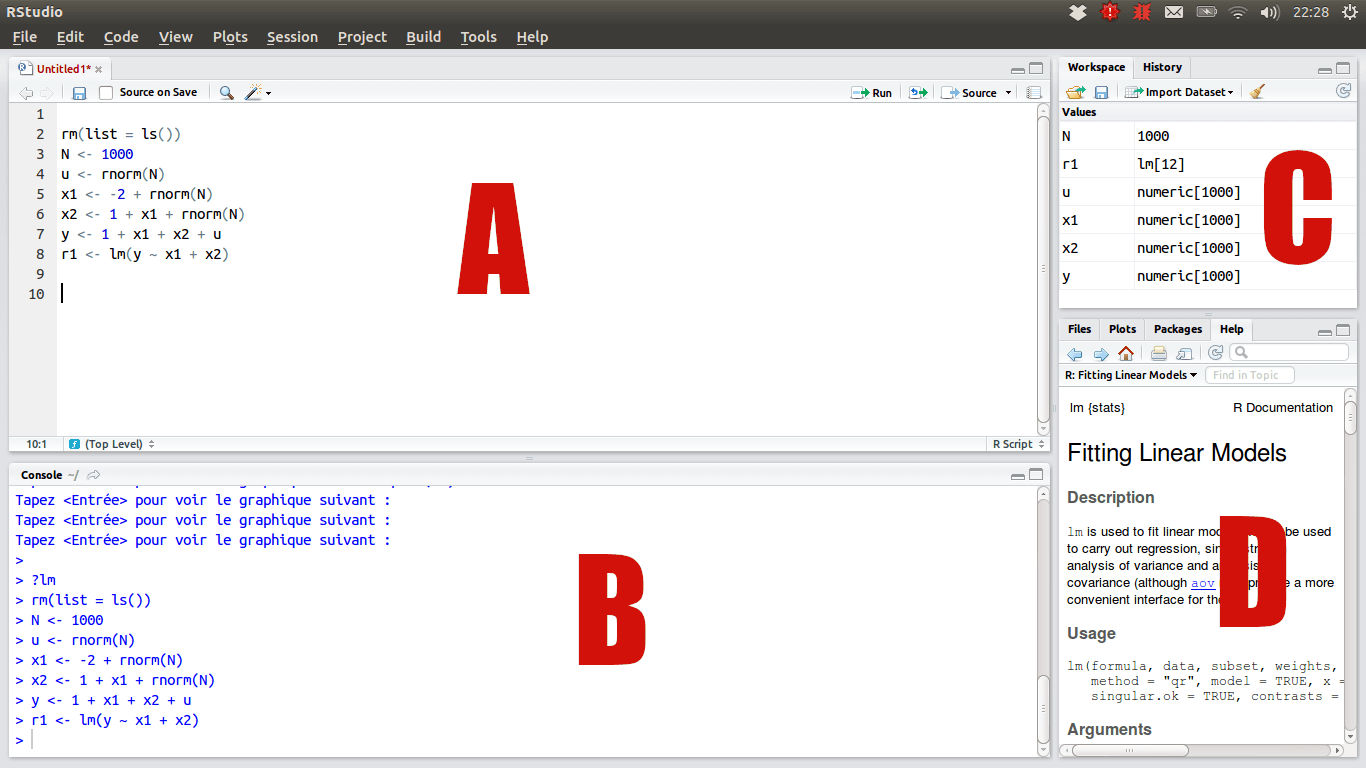
\includegraphics[scale=0.65]{Rstudio_interface1}
	\end{column}
	\begin{column}{0.4\textwidth}
	\begin{enumerate}
		\item[A] Skriptfenster
		\item[B] Konsole / Eingabezeile
		\item[C] Workspace, Daten
		\item[D] Plots, Hilfe, Dateibrowser, Paketmanager
	\end{enumerate}
	\end{column}
\end{columns}
\end{frame}
\begin{frame}{Eingabezeile und Taschenrechner}
	\begin{columns}[T]
	\begin{column}{0.6\textwidth}
	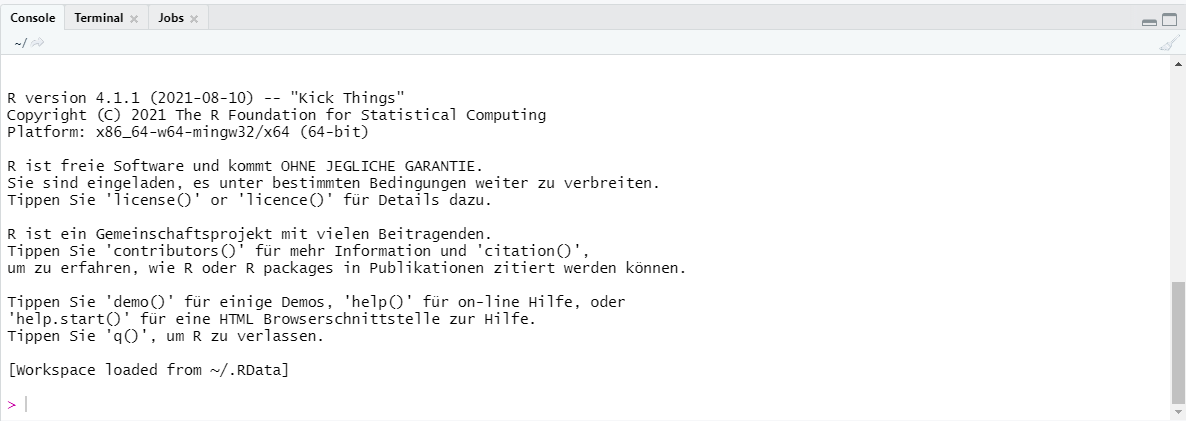
\includegraphics[width=\textwidth]{Rstudio_interface_c}
	\end{column}
	\begin{column}{0.4\textwidth}
	\begin{itemize}
		\item Nur \glqq Console\grqq{} relevant
		\item In der Konsole kann man Befehle eintippen und  mit Enter ausführen
		\item Beispiel Taschenrechner:
		\begin{itemize}
			\item 3 + 2
			\item 5 * 4
			\item 20 - 8
			\item 12 / 16
		\end{itemize}
	\end{itemize}
	\end{column}
\end{columns}
\end{frame}

\begin{frame}[fragile]{Fehler, Warnungen, NA, NaN, Inf}
	Was passiert, wenn wir \verb+ 5!+ eintippen? \\
	R gibt uns einen Fehler zurück. Es ist wichtig, dass wir wissen, wie wir R einen Befehl mitteilen. Also: \verb+ factorial(5)+. \\
	\begin{itemize}
		\item 3 / 0 $\Rightarrow$ \verb+ Inf+; R löst die Aufgabe numerisch und landet bei einem Grenzwert (hier \verb+ Inf+ $=\infty$).
		\item 0/0 $\Rightarrow$ \verb+ NaN+; Steht für \glqq Not a Number\grqq{}
		\item NA steht einfach für einen fehlenden Wert. Dies tritt vor allem auf, wenn bei einer Operation nicht angegeben wurde, wie mit vorhandenen fehlenden Werten umgegangen werden soll.
		
	\end{itemize}

\end{frame}

\begin{frame}[fragile]{Mathematische Ausdrücke}
	\begin{itemize}
		\item \verb+ factorial(x)+ $= x!$
		\item \verb+ exp(x)+ $=e^x$
		\item \verb+ log(x)+ $=log(x)$
		\item \verb+ sqrt(x)+ $=\sqrt{x}$
		\item \verb+ abs(x)+ $=\abs{x}$
	\end{itemize}
\end{frame}

\begin{frame}{Skriptfenster}
	\begin{columns}[T]
	\begin{column}{0.6\textwidth}
	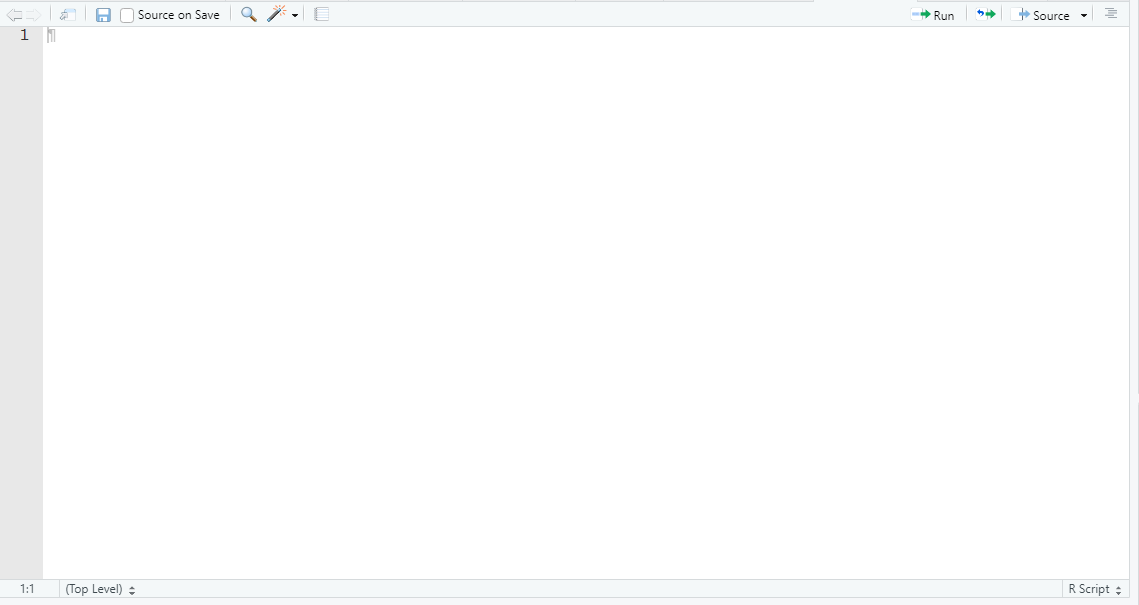
\includegraphics[width=\textwidth]{Rstudio_interface_i}
	\end{column}
	\begin{column}{0.4\textwidth}
	\begin{itemize}
		\item Es ist umständlich, Befehl für Befehl in die Konsole zu schreiben
		\item Im Skriptfenster können wir beliebig viele Befehle nacheinander reinschreiben und ganze Blöcke auf einmal ausführen
		\item Technisch passiert beim Ausführen eines Skripts nichts anderes, als dass Zeile für Zeile an die Konsole übergeben wird
		\item Skripte lassen sich speichern und wiederverwenden
	\end{itemize}
	\end{column}
\end{columns}
\end{frame}

\begin{frame}[fragile]{Variablen zuweisen}
Oft wollen wir Ergebnisse oder Daten irgendwo speichern, um sie später weiterverwenden zu können. Dazu müssen wir Variablen zuweisen. In R wird dazu (historisch) ein Pfeil verwendet: \verb+ <-+. Genauso funktioniert allerdings das \verb+ =+ um Daten zuzuweisen. Variablen sind \glqq Case Sensitive\grqq{}, d.h. Groß- und Kleinschreibung ist wichtig!
\begin{itemize}
	\item \verb+ x <- 3.1415+
	\item \verb+ b <- 4+
	\item \verb+ B = 5+
	\item \verb+ d <- c(1,2,5,7)+
\end{itemize}
\end{frame}

\begin{frame}[fragile]{Sonstiges}
R bietet einige nützliche Funktionen. Zwei besonders nützliche sind \verb+?+ und \verb+rm(x)+.
\begin{itemize}
	\item Wenn wir wissen wollen, was eine Funktion macht, können wir mit dem Fragezeichen gefolgt vom Namen der Funktion ihre Dokumentation aufrufen. Z.B.: \verb+?rm+
	\item Wenn wir das nun eingeben, erfahren wir direkt mehr über die zweite nützliche Funktion: Wir können in die Klammern Objekte reinschreiben, die wir löschen wollen. Von der vorherigen Folie haben wir noch \verb+x+, \verb+b+, \verb+B+ und \verb+d+
	\item Wir wollen nun \verb+B+ und \verb+b+ löschen, also: \verb+ rm(B, b)+
\end{itemize}
\end{frame}

%% ================================================================== %%
\section{Daten}
\begin{frame}[fragile]{Datentypen}
	Welche Arten von Daten gibt es in R?
	\begin{itemize}
		\item Numeric $\Leftrightarrow$ Zahlen, \verb+is.numeric()+
		\item Character $\Leftrightarrow$ Buchstaben/Wörter \verb+is.character()+
		\item Factor $\Leftrightarrow$ Kategorische Variablen \verb+is.factor()+
		\item Date $\Leftrightarrow$ Datum/Zeit \verb+is.Date()+
	\end{itemize}
\end{frame}

\begin{frame}[fragile]{Vektor}
	R ist eine Vektor-Sprache: Fast alle Datenkonstruktionen sind Formen oder Erweiterungen eines Vektors. \\
	Ein R-Vektor kann nur einen Datentypen beinhalten.
	\begin{itemize}
		\item \verb+ c()+
		\item \verb+ seq()+
		\item \verb+ rep()+
		\item \verb+ is.vector()+
	\end{itemize}
\end{frame}

\begin{frame}[fragile]{Matrix}
	Eine Matrix ist eine Aneinanderreihung von Vektoren (nebeneinander, untereinander). \\
	Eine R-Matrix kann nur einen Datentypen beinhalten.
	\begin{itemize}
		\item \verb+ matrix()+
		\item \verb+ cbind()+
		\item \verb+ rbind()+
		\item \verb+ is.matrix()+
	\end{itemize}
\end{frame}

\begin{frame}[fragile]{Rechenoperationen}
Man kann in R einfach mit Vektoren und Matrizen rechnen.  Grundsätzlich: Elementweise! Was erhält man bei folgendem Befehl? \\
\verb+ c(3.1415, 5, 1, 2/3) * seq(1, 8, 2)+ \\
R rechnet folgendermaßen: \begin{align*}
	\begin{pmatrix}
	3.1415 \\ 5 \\ 1 \\ \frac{2}{3}
	\end{pmatrix} \quad * 
	\underbrace{\begin{pmatrix}
		1 \\ 3 \\ 5 \\ 7
	\end{pmatrix}}_{\text{seq(1, 8, 2) = c(1, 3, 5, 7)}}
	\quad &= \quad \begin{pmatrix}
	3.1415 \cdot 1 \\
	5 \cdot 3 \\
	1 \cdot 5 \\
	\frac{2}{3} \cdot 7
	\end{pmatrix}
\end{align*}
\end{frame}

\begin{frame}[fragile]{Liste}
	Was, wenn wir verschiedene Datentypen in einem Vektor speichern wollen? \\
	Antwort: Liste.\\
	Listen sind etwas abstraktere Varianten des klassischen Vektors, da Listenelemente nicht den gleichen Datentyp haben müssen. Listen sind flexibel und können sogar verschachtelt werden, also eine Liste kann weitere Listen enthalten.
	\begin{itemize}
		\item \verb+ list()+
		\item \verb+ c()+
		\item \verb+ $ +
	\end{itemize}
\end{frame}

\begin{frame}[fragile]{Data Frame}
	Listen sind manchmal etwas unübersichtlich. Eine spezielle Form einer Liste ist der Data Frame.\\
	Optisch sieht der Data Frame aus wie eine Matrix, allerdings können hier unterschiedliche Datentypen gespeichert werden. Unterschiedliche Spalten (nur Spalten, keine Zeilen) können vom unterschiedlichen Typ sein.
	\begin{itemize}
		\item \verb+ data.frame()+
		\item \verb+ rbind()+
		\item \verb+ cbind()+
		\item \verb+ $+
	\end{itemize}
\end{frame}

\section{Speichern von Daten}

\begin{frame}[fragile]{Speichern}
	Oft kommt es vor, dass wir nicht nur einmal an etwas arbeiten. Es macht also Sinn, Daten zu speichern. Unter anderem bietet R einen Dateityp an, mit dem man R-Daten speichern kann: \verb+ *.RData+
	\begin{itemize}
		\item \verb+ save()+
		\item \verb+ write.table()+
		\item \verb+ write.csv()+
	\end{itemize}
\end{frame}

\end{document}
%% ================================================================== %%
%% ================================================================== %% 
